\documentclass[a4paper]{article}

%use the english line for english reports
%usepackage[english]{babel}
\usepackage[portuguese]{babel}
\usepackage[utf8]{inputenc}
\usepackage{indentfirst}
\usepackage{graphicx}
\usepackage{verbatim}
\usepackage{fancyhdr}
\usepackage{listings}

\usepackage{listings}
\usepackage{color}

\definecolor{dkgreen}{rgb}{0,0.6,0}
\definecolor{gray}{rgb}{0.5,0.5,0.5}
\definecolor{mauve}{rgb}{0.58,0,0.82}

\lstset{frame=tb,
  language=Prolog,
  aboveskip=3mm,
  belowskip=3mm,
  showstringspaces=false,
  columns=flexible,
  basicstyle={\small\ttfamily},
  numbers=none,
  numberstyle=\tiny\color{gray},
  keywordstyle=\color{blue},
  commentstyle=\color{dkgreen},
  stringstyle=\color{mauve},
  breaklines=true,
  breakatwhitespace=true,
  tabsize=3
}

\begin{document}

\setlength{\textwidth}{16cm}
\setlength{\textheight}{22cm}

\title{\Huge\textbf{FABRIK}\linebreak\linebreak\linebreak
\Large\textbf{Relatório Intercalar}\linebreak\linebreak
\linebreak\linebreak

\includegraphics[scale=0.1]{images/feup-logo.png}\linebreak\linebreak
\linebreak\linebreak
\Large{Mestrado Integrado em Engenharia Informática e Computação} \linebreak\linebreak
\Large{Programação em Lógica}\linebreak
}

\author{\textbf{Grupo Fabrik3:}\\
\linebreak\\
André Cruz - 201503776 \\
Edgar Carneiro - 201503778 \\
\linebreak\linebreak \\
 \\ Faculdade de Engenharia da Universidade do Porto \\ Rua Roberto Frias, s\/n, 4200-465 Porto, Portugal \linebreak\linebreak\linebreak
\linebreak\linebreak\vspace{1cm}}

\maketitle
\thispagestyle{empty}

%************************************************************************************************
%************************************************************************************************

\newpage

%Todas as figuras devem ser referidas no texto. %\ref{fig:codigoFigura}
%
%%Exemplo de código para inserção de figuras
%%\begin{figure}[h!]
%%\begin{center}
%%escolher entre uma das seguintes três linhas:
%%\includegraphics[height=20cm,width=15cm]{path relativo da imagem}
%%\includegraphics[scale=0.5]{path relativo da imagem}
%%\includegraphics{path relativo da imagem}
%%\caption{legenda da figura}
%%\label{fig:codigoFigura}
%%\end{center}
%%\end{figure}
%
%
%\textit{Para escrever em itálico}
%\textbf{Para escrever em negrito}
%Para escrever em letra normal
%``Para escrever texto entre aspas''
%
%Para fazer parágrafo, deixar uma linha em branco.
%
%Como fazer bullet points:
%\begin{itemize}
	%\item Item1
	%\item Item2
%\end{itemize}
%
%Como enumerar itens:
%\begin{enumerate}
	%\item Item 1
	%\item Item 2
%\end{enumerate}
%
%\begin{quote}``Isto é uma citação''\end{quote}

%Index
\tableofcontents
\newpage

%%%%%%%%%%%%%%%%%%%%%%%%%%
\section{O Jogo\textit{Fabrik}}

\subsection{História}
O jogo - \textit{Fabrik} - foi recentemente desenvolvido por Dieter Stein, em Agosto de 2017, como parte de um estudo para o desenvolvimento de um novo jogo, Urbino.

\subsection{Material}
\begin{itemize}
	\item Tabuleiro quadrangular
	\item Quantidade suficiente de peças pretas e brancas
	\item Duas peças vermelhas chamadas trabalhadores
\end{itemize}

\begin{figure}[h!]
\begin{center}
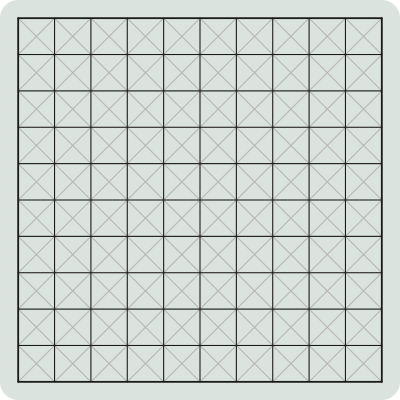
\includegraphics[height=3cm,width=3cm]{images/fabrik_empty_board.png}
\caption{Tabuleiro vazio de 11 x 11 espaços}
\label{Figura 1}
\end{center}
\end{figure}

\subsection{Regras}
As pretas (jogador que joga com peças de cor preta) começam por colocar um dos trabalhadores num espaço à sua escolha. De seguida, as brancas (jogador que joga com peças de cor branca) coloca o outro trabalhador num espaço qualquer. As pretas decidem quem começa por jogar.
O jogo funciona por turnos sendo que em cada um turno um jogador pode, se assim optar, mexer um dos trabalhadores para um espaço vazio. De seguida, o jogador deve jogar uma das suas  peças e coloca-la num ponto de interseção entre as “linhas de visão dos dois trabalhadores”. As linhas de visão dos trabalhadores são as linhas na diagonal, horizontal e vertical sobre as quais os trabalhadores se encontram posicionados.

\begin{figure}[h!]
\begin{center}
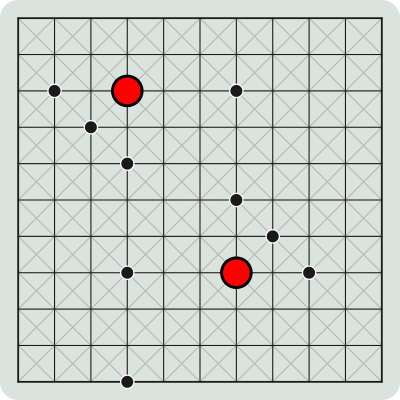
\includegraphics[height=3cm,width=3cm]{images/fabrik_intersection.png}
\caption{Pontos de interseção entre os dois trabalhadores}
\label{Figura 2}
\end{center}
\end{figure}

No caso especial em que os dois trabalhadores se encontram sobre uma mesma linha ortogonal ou diagonal, apenas os espaços entre eles são considerados pontos de interseção (se estiverem vazios), ao invés da totalidade dessa linha.
Ganha o jogo o jogador que consiga criar uma linha de pelo menos 5 pedras da sua cor, ortogonalmente ou diagonalmente. Um jogador ganha também o jogo se o seu adversário não conseguir posicionar nenhum dos trabalhadores de forma a poder colocar uma pedra sua no tabuleiro.

\begin{figure}[h!]
\begin{center}
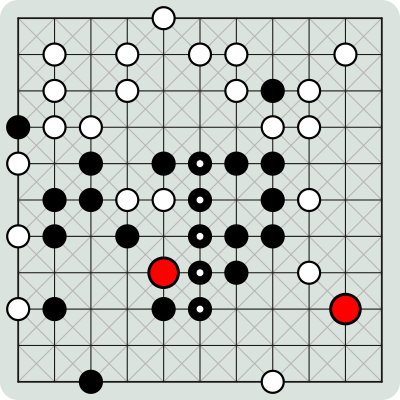
\includegraphics[height=3cm,width=3cm]{images/fabrik_full_board.png}
\caption{Final de uma partida de Fabrik, com vitórias das pretas}
\label{Figura 3}
\end{center}
\end{figure}

\vfill
\textbf{Referências:}\newline
https://spielstein.com/games/fabrik\newline
https://spielstein.com/games/fabrik/rules



\newpage

\section{Modelação do Jogo em Prolog}
%%%%%%%%%%%%%%%%%%%%%%%%%%
\subsection{Representação do Estado do Jogo}

A representação dos estados de jogo é feita com recurso a uma lista de listas, de forma a simular o uso de uma Matriz. Seguem de seguida, a representaçao de diferentes estados de jogo:\newline



Representação do \textbf{estado inicial}:

\begin{small}
\begin{lstlisting}
[[none, none, none, none,  none, none,  none, none, none, none, none],
 [none, none, none, none,  none, none,  none, none, none, none, none],
 [none, none, none, none,  none, none,  none, none, none, none, none],
 [none, none, none, none,  none, none,  none, none, none, none, none],
 [none, none, none, none,  none, none,  none, none, none, none, none],
 [none, none, none, none,  none, none,  none, none, none, none, none],
 [none, none, none, none,  none, none,  none, none, none, none, none],
 [none, none, none, none,  none, none,  none, none, none, none, none],
 [none, none, none, none,  none, none,  none, none, none, none, none],
 [none, none, none, none,  none, none,  none, none, none, none, none],
 [none, none, none, none,  none, none,  none, none, none, none, none]]
\end{lstlisting}
\end{small}

\begin{figure}[h!]
\centering
\begin{minipage}{.35\textwidth}
	\centering
	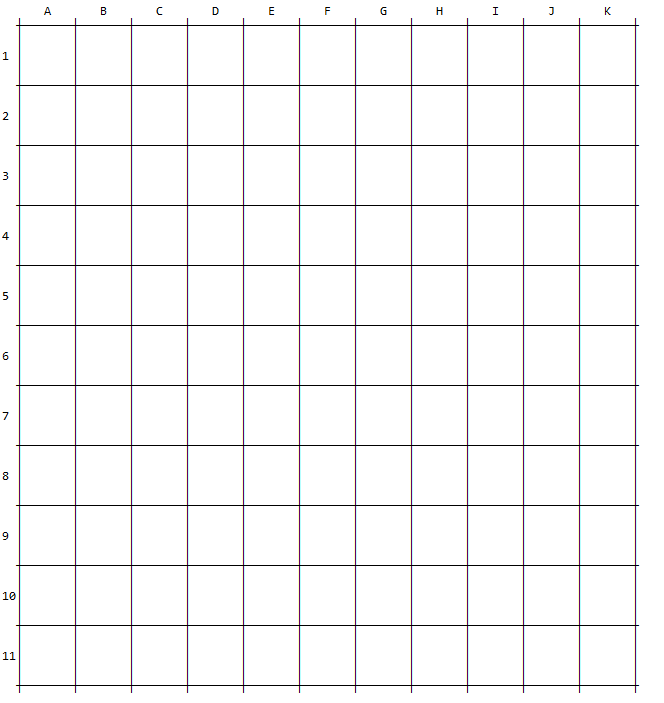
\includegraphics[width=\textwidth]{images/self_empty_board.png}
	\caption{Representação do estado inicial na consola}
	\label{Figura 4}
\end{minipage}
\quad \quad
\begin{minipage}{.35\textwidth}
	\centering
	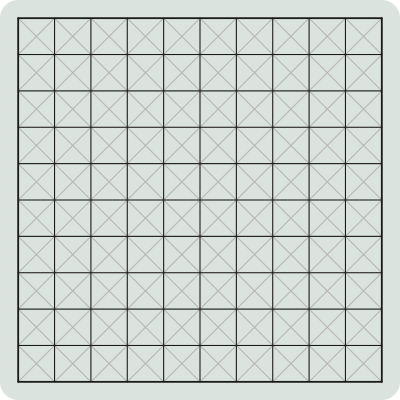
\includegraphics[width=\textwidth]{images/fabrik_empty_board.png}
	\caption{Tabuleiro original Vazio}
	\label{Figura 5}
\end{minipage}
\end{figure}

\clearpage

Representação de um possível \textbf{estado intermédio}:\newline

\begin{small}
\begin{lstlisting}
[[ none, none, none, none, none, none, none, none, none, none, none],
 [ none, none, none, none, none, white, worker, none, none, none, none],
 [ none, none, none, none, none, none, white, black, white, none, none],
 [ none, white, white, none, none, none, none, white, white, none, none],
 [white, none, none, none, black, black, none, black, none, none, none],
 [ none, none, black, white, none, none, none, none, white, none, none],
 [ none, black, none, none, none, black, black, black, none, none, none],
 [ none, none, none, none, none, none, black, none, white, none, none],
 [ none, none, none, none, none, black, none, none, none, none, none],
 [ none, none, none, none, worker, none, none, none, none, none, none],
 [ none, none, none, none, none, none, none, none, none, none, none]]
\end{lstlisting}
\end{small}

\begin{figure}[h!]
\begin{center}
	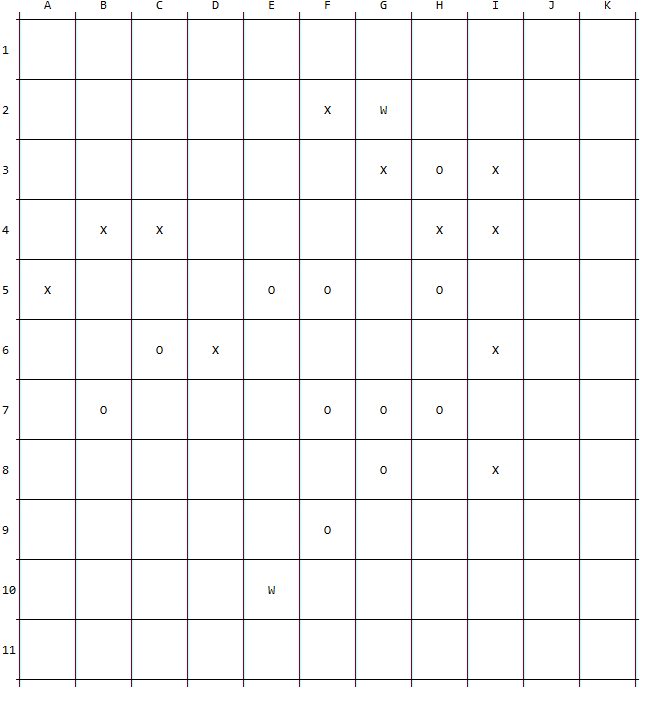
\includegraphics[height=6cm, width=6cm]{images/self_semi_board.png}
	\caption{Representação na consola, de um possível estado intermédio}
	\label{Figura 6}
\end{center}
\end{figure}

\clearpage
Representação de um possível \textbf{estado final}:\newline

\begin{small}
\begin{lstlisting}
[[ none, none, none, none, white, none, none, none, none, none, none],
 [ none, white, none, white, none, white, white, none, none,white, none],
 [ none, white, none, white, none, none,white, black, white, none, none],
 [black, white, white, none, none, none, none, white, white, none, none],
 [white, none, black, none,black, black, black, black, none, none, none],
 [none, black, black, white,white, black, none, black,white, none, none],
 [white, black, none,black, none, black, black, black, none, none, none],
 [ none, none, none, none, worker, black, black, none,white, none, none],
 [white, black, none, none,black, black, none, none, none, worker, none],
 [ none, none, none, none, none, none, none, none, none, none, none],
 [ none, none, black, none, none, none, none, white, none, none, none]]
\end{lstlisting}
\end{small}

\begin{figure}[h!]
\centering
\begin{minipage}{.35\textwidth}
	\centering
	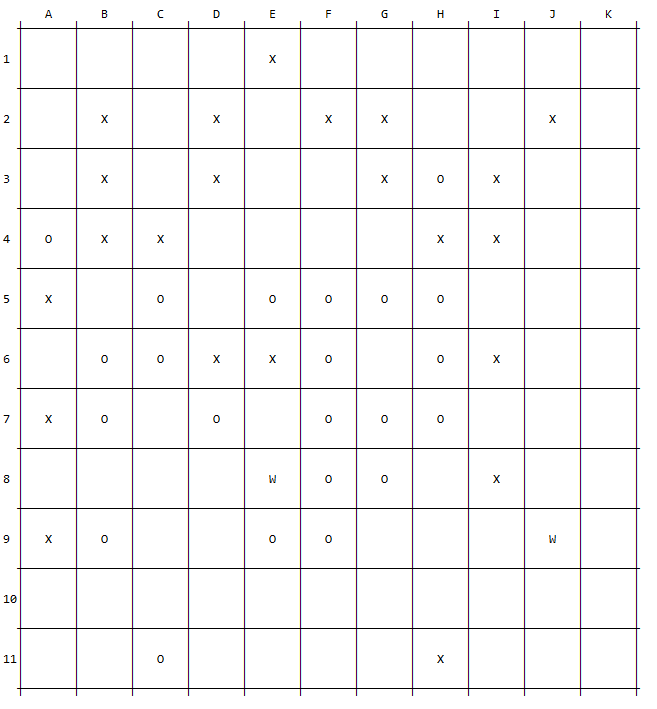
\includegraphics[width=\textwidth]{images/self_full_board.png}
	\caption{Representação do estado final na consola}
	\label{Figura 7}
\end{minipage}
\quad \quad
\begin{minipage}{.35\textwidth}
	\centering
	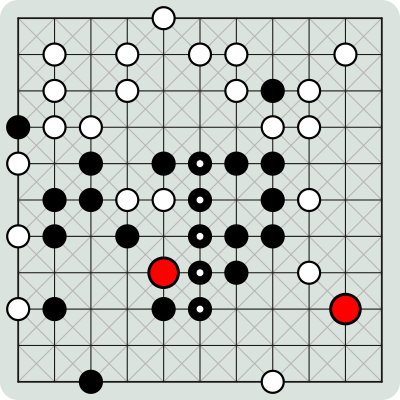
\includegraphics[width=\textwidth]{images/fabrik_full_board.png}
	\caption{Representção do mesmo estado final, no tabuleiro original}
	\label{Figura 8}
\end{minipage}
\end{figure}

\clearpage


%%%%%%%%%%%%%%%%%%%%%%%%%%
\subsection{Visualização do Tabuleiro}

Para a representação do tabuleiro em modo de texto, foi criado o seguinte código em prolog:
\begin{lstlisting}[language=prolog]
% Board Printing - Character Translation
translate(none, Symbol) :- Symbol = ' '.
translate(black, Symbol) :- Symbol = 'O'.	% Dark Pieces
translate(white, Symbol) :- Symbol = 'X'.	% White Pieces
translate(worker, Symbol) :- Symbol = 'W'.% Red Workers

% Board Printing - arguments: Board and Board size
printFabrik(Board, N):-
        nl, 
        write('  '), printHorizontalLabel(N, N),
        printBoard(Board, N, 1).

printBoard([], N, _):-
        printRowDivider(N), nl.

printBoard([Line | Board], N, CurrentL) :-
        printRowDivider(N),
        printDesignRow(N),
        printVerticalLabel(CurrentL),
        put_code(9474),
        printLine(Line),
        printDesignRow(N),
        NewL is (CurrentL+1),
        printBoard(Board, N, NewL).

printLine([]) :- nl.
printLine([Head | Tail]) :-
        translate(Head, Symbol),
        write('   '),
        write(Symbol),
        write('   '), put_code(9474),
        printLine(Tail).

%              AESTHETICS

printRowDivider(N):-
        write('  '),
        put_code(9532),
        printRowDividerRec(N).

printRowDividerRec(0) :- nl.
printRowDividerRec(N) :-
        put_code(9472), put_code(9472), put_code(9472), put_code(9472),
        put_code(9472), put_code(9472), put_code(9472), put_code(9532),
        N1 is (N-1),
        printRowDividerRec(N1).

printDesignRow(N):-
        write('  '),
        put_code(9474),
        printDesignRowRec(N).

printDesignRowRec(0) :- nl.
printDesignRowRec(N) :-
        write('       '), put_code(9474),
        N1 is (N-1),
        printDesignRowRec(N1).

% Dictionary for Labels
getLabel(0, L):- L = 'A'.
getLabel(1, L):- L = 'B'.
getLabel(2, L):- L = 'C'.
getLabel(3, L):- L = 'D'.
getLabel(4, L):- L = 'E'.
getLabel(5, L):- L = 'F'.
getLabel(6, L):- L = 'G'.
getLabel(7, L):- L = 'H'.
getLabel(8, L):- L = 'I'.
getLabel(9, L):- L = 'J'.
getLabel(10, L):- L = 'K'.
getLabel(11, L):- L = 'L'.

printHorizontalLabel(0, _):- nl.
printHorizontalLabel(N, Total):-
        Pos is (Total-N),
        getLabel(Pos, L),
        write('    '), write(L), write('   '),
        N1 is (N-1),
        printHorizontalLabel(N1, Total).        

printVerticalLabel(CurrentL):-
        CurrentL < 10,
        write(CurrentL),
        write(' ').

printVerticalLabel(CurrentL):-
        write(CurrentL).
\end{lstlisting}

Representação de um tabuleiro, usando o código mencionado:\newline

\begin{figure}[h!]
\begin{center}
	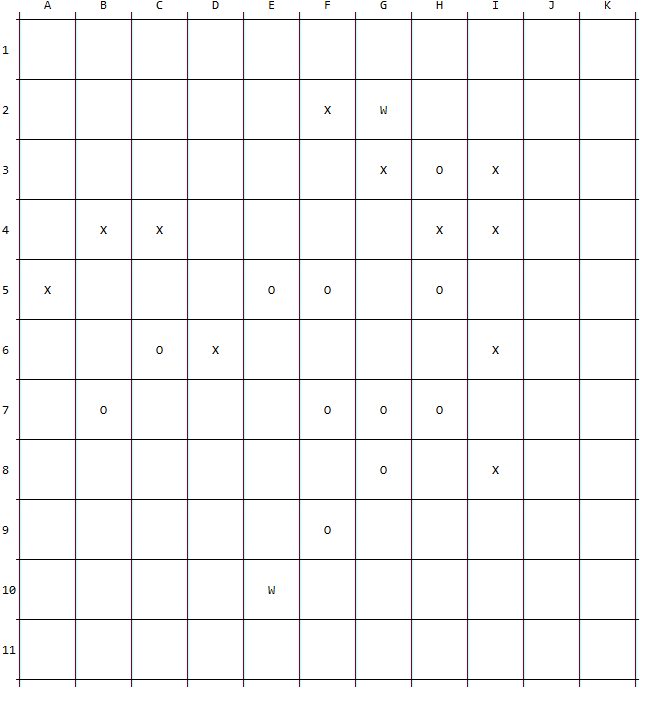
\includegraphics[height=4cm, width=4cm]{images/self_semi_board.png}
	\caption{Representação de um tabuleiro na consola}
	\label{Figura 9}
\end{center}
\end{figure}

\newpage

%%%%%%%%%%%%%%%%%%%%%%%%%%
\subsection{Movimentos}
Os predicados que consideramos serem necessários definir para os movimentos associados ao jogo são:

\begin{itemize}
	\item \textit{putPiece(Row, Col, Board, PieceType)}\newline
	Colocação de uma peça, branca ou preta, no tabuleiro, na posição [Row, Col].
	
	\item \textit{moveWorker(Row, Col, DestRow, DestCol, Board)}\newline
	Movimentação da peça '\textit{trabalhador}' na posição [Row, Col] para a posição [DestRow, DestCol]
\end{itemize}
	

\end{document}
